\subsection{Kommunikation} \label{grund-kommunikation}


Da insbesondere bei der Messung von EEG,EOG und GSR relativ kleine Spannungsunterschiede betrachtet werden, ist es wichtig gerade diese analogen Signale wenig zu beeinträchtigen. Diese Signale werden mittels Elektroden gemessen. Ziel war es also eine möglichst Störungsfreie Kommunikation zum einen zwischen den einzelnen Sensoren und der PCB als auch zwischen der PCB und einen Computer, auf dem die Rohdaten verarbeitet werden sollen, zu ermöglichen. Um die Einwirkung von Rauschen auf die oben genannten analogen Signale schon von vorneherein zu minimieren, wurde die Übertragungsstrecke zwischen Elektroden und PCB in späteren Versionen so kurz wie möglich gehalten. Alle analogen Signale werden dann in digitale Signale umgewandelt, und direkt Drahtlos an einen empfangenden Rechner gesendet, der die Daten zur späteren Bearbeitung abspeichert. Die Drahtlose Übertragung wurde in der ursprünglichen Variante mittels Bluetooth realisiert, wobei die Daten am empfangenden Rechner mittels Serialplot direkt visualisiert, und dann auch abgespeichert wurden. Bei dieser visuellen Darstellung, werden die Rohdaten lediglich auf einer Zeitachse aufgetragen. Der Vorteil dabei ist, dass sofort eine zumindest grobe Einschätzung, ob die Daten korrekt sind, möglich ist.


% Unterkapitel
\subsection{Serial-Peripheral Interface(SPI)} \label{grund-spi-subsubsec}

\todo[inline]{Verantwortlich: Kevin, Jonas}

Das Serial Peripheral Interface (kurz: SPI) ist ein, in 1987 entwickeltes Bussystem, das aus drei Leitungen für eine serielle und synchrone Datenübertragung zwischen verschiedenen ICs besteht. Dieses Bussystem stellt einen Verbindungsstandard für einen synchronen seriellen Datenbus dar. Mit diesem Standard können unterschiedliche digitale Schaltungen nach einem Master-Slave Prinzip miteinander verbunden werden.

 MOSI (Master Out  Slave In) auch SDO (Serial Data Out)
 MISO (Master In   Slave Out) auch SDI (Serial Data In)
 SCK (Serial Clock) – Schiebetakt

Außerdem wird noch eine weitere Leitung benötigt, welche Slave Select (SS) oder auch
Chip Select (CS) genannt wird, durch die der Master jeden verbundenen Slave zur aktuellen
Kommunikation selektiert. Die Auswahl erfolgt hierbei vom Master durch den Wechsel des
High-Pegels auf der SS/CS-Leitung nach Low. Zusätzlich kann der Master dem Slave eine
Benachrichtigung durch verändern des Pegels anzeigen, die diesem mitteilt, dass eine neue
Nachricht übertragen wird. Nachrichten haben hier eine Größe von mindestens einem Byte.

\begin{figure}[H] \centering
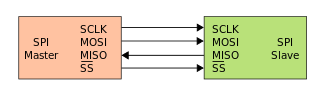
\includegraphics[width=\textwidth]{Images/SPI_single_slave.png} 
\vspace{-0.3cm} 
\caption{ SPI-Kommunikation zwischen einem einzelnen Master und Slave.}
\label{fig-elise} 
\end{figure}

Der SPI-Bus wird ohne ein festgelegtes Protokoll betrieben. Jedoch müssen für einen reibungslosen
Betrieb die Einstellungen des Schiebetaktes vom Master auf der SCK-Leitung an
die Spezifikationen und Anforderungen des Slaves angepasst werden, da sowohl die Taktpolarität
(CPOL) und Phase (CPHA) von Slave zu Slave unterschiedlich sein können. Die Übertragung erfolgt dabei in verschiedenen Zyklen. Der Master bringt seine Datenleitung zum Senden (MOSI) auf den Pegel des nächsten Bits, das übertragen werden soll. Da der Master den Kommunikationszyklus initialisiert, gibt er auf der SCK-Leitung einen Puls aus. Um Daten des Slaves als Antwort zu erhalten, muss der Master während seines Sendevorgangs den
Pegel an der Datenleitung vom Slave zum Master (MISO) überwachen. Der Zustand dieser
Datenleitung wird als nächstes einzulesendes Bit aufgefasst. Um den Grundzustand der SCK-Leitung zu konfigurieren, also die Flanke des Taktes zur Datenübernahme einzustellen, muss die Taktpolarität (CPOL) und Phase (CPHA) an den Slave angepasst werden. In manchen Fällen kann diese Konfiguration auch auf vereinzelten Slaves vorgenommen werden.

\begin{figure}[H] \centering
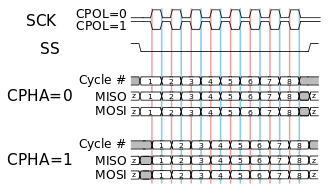
\includegraphics[width=\textwidth]{Images/SPI_timing_diagram2.png} 
\vspace{-0.3cm} 
\caption{Datenübertragung für verschieden CPOL und CPHA.}
\label{fig-elise} 
\end{figure}

% Unterkapitel
\subsection{Inter-Intergrated Circuit (I2C)} \label{grund-i2c-subsubsec}

\todo[inline]{Verantwortlich: Kevin, Jonas}

Das Inter-Integrated Circuit (kurz: I2C, gesprochen I-Quadrat-C), oder auch Inter IC-Bus, ist wie das in Kapitel 2.1. besprochene SPI ein synchrones und serielles Bussystem. Dieses wurde 1982  von Philips entwickelt und ermöglicht eine Kommunikation zwischen verschiedenen integrierten Schaltungen (ICs, engl. Integrated Circuit) für die nur zwei Leitungen benötigt werden. Das Protokoll erlaubt es bei einer Adressierung von sieben Bit, mit bis zu 128 Slaves zu kommunizieren. Vorteil dieses Bussystems ist die Kommunikation mit einem oder mehreren Master ICs. Ein I2C-Bus mit mehreren Master ICs wird als "Multi-Master-Bus"bezeichnet. Die Übertragungsraten bei Mikrocontrollern betragen bis zu 400 kbit/s und können in leistungsstärkeren Systemen bis zu 3,4 MBit/s erreichen. Taktgeschwindigkeiten sollten sich aber immer am langsamsten IC im Bus orientieren, damit es nicht zu kommunikationsproblemen kommt. Slaves sind mit einer eigenen, individuellen fest zugeordneten Adresse codiert. Über einen Broadcastkanal können analog alle Slaves in einem Verbund gleichzeitig angesprochen werden. Die Adressierung erfolgt dabei stehts durch den Master. Das heißt, dass Slaves niemals selbständig eine Kommunikation starten können. Lediglich der Master teilt nach Versenden der Slave-Adresse mit (Adresse ist dabei sieben Bit lang), ob er im Folgenden Daten senden oder von dem jeweiligen Gerät empfangen möchte (das 8. Bit), die dann entweder vom Master oder vom Slave auf den Bus gelegt werden. Also initiert der Master den Datentransfer und synchronisiert den Takt, mit dem der Transfer abläuft. Nach erfolgreicher Kommunikation gibt der Master den Bus anschließend wieder frei. Betrachtet man die Kommunikation auf Bitebene, werden durch eine Kombination der Zustände von Takt- und Datenleitung die Start-/Stopp-Bedingungen durch den Master eingeleitet. Um die erfolgreiche Kommunikation zwischen Master und Slave sicherzustellen, wird für die Quittierung zwischen einzelnen Datenpaketen und nach Übertragung der gesamten Daten ein Acknowledge bzw. Not-Acknowledge versendet.

\begin{figure}[H] \centering
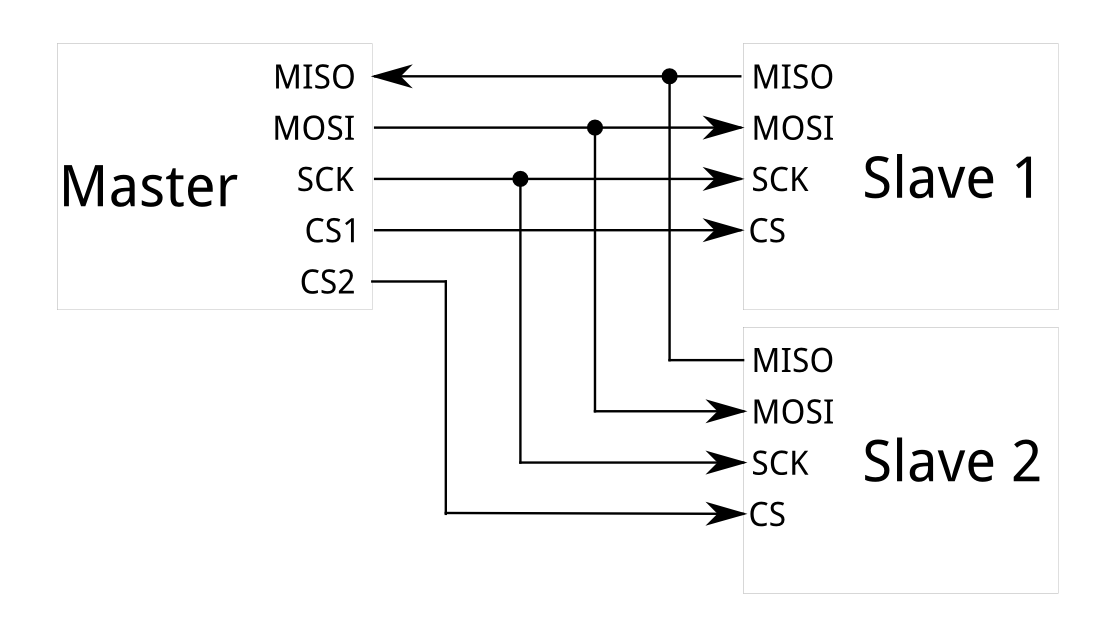
\includegraphics[width=\textwidth]{Images/I2C_multiple_slaves.png} 
\vspace{-0.3cm} 
\caption{ I2C-Master mit 2 Slaves.}
\label{fig-elise} 
\end{figure}

% Unterkapitel
\subsection{Bluetooth} \label{grund-bluetooth-subsubsec}

\todo[inline]{Verantwortlich: Kevin, Jonas}

Der in den 1990er Jahren durch die Bluetooth Special Interest Group entwickelte Industriestandard (gemäß IEEE802.15.1) definiert die Datenübertragung zwischen Geräten mittels Funktechnik(WPAN). Mit Bluetooth können Geräte drahtlos und ohne direkte Sichtverbindung über kurze Distanzen miteinander kommunizieren. Der Name Bluetooth bezieht sich auf den dänischen König Harald II. Blaatand (übersetzt Blauzahn, englisch Bluetooth), der verfeindete Teile von Norwegen und Dänemark vereinte. So sollte auch diese Funktechnik die Computer- und Telekommunikations-Welt zusammenführen und dadurch eine Vielzahl unterschiedlicher Anschlüsse ablösen sollte. Bluetooth definiert einen vollständigen Protokollstapel bis zur Anwendungsschicht. Somit erfolgt die Zusammenarbeit der Geräte auf der Anwendungsebene und definiert zudem unterschiedliche  Profile für verschiedene Anwendungsbereiche, wie zum Beispiel Netzverwaltung, verbindungsorientierter oder –loser Dienst, Dienst-Abfragen, Telefondienste, usw..
Es gibt für Bluetooth eine Vielzahl unterschiedlicher Anwendungsfälle. Zum einen die Vernetzung mobiler Endgeräte, wie z.B. Smartphones, Ein- und Ausgabegeräte, PCs, Notebooks aber auch Mikrocontroller, zum Austausch von Daten und wichtiger Informationen. Zum anderen vor allem in der heutigen Zeit zwischen Smartphones und Audiogeräten. Die Übertragung läuft dabei über logische Kanäle (sogenannte Links) und erfolgt entweder asynchron, das heißt verbindungslos nach dem best effort-Prinzip, oder synchron, das heißt verbindungsbehaftet zur Echtzeitübertragung nach dem guaranteed timeliness-Prinzip. Die Kommunikation ist von Punkt zu Punkt, Ad-hoc- bis hin zu Piconetzen möglich und wird durch einen Master durch Vergabe von Sende-Zeitschlitzen (Zeitmultiplexverfahren), dem sogenannten Frequenzsprung-Spread-Spectrum-Verfahren (Frequency Hopping Spread Spectrum, FHSS), gesteuert. In dem Frequenzsprungverfahren beträgt die nominale Sprungrate 1600 Hops pro Sekunde. Aus der Sprungrate ergibt sich ein Zeitschlitz mit einer Länge von 625 %μs 
für jeden Slave, wobei eine Übertragung von allen Teilnehmern nur zu Beginn eines Zeitschlitzes gestartet werden darf. Die Frequenzfolge ist pseudozufällig und somit in jedem Piconetz unterschiedlich. Auf diese Weise soll der Betrieb von möglichst vielen unabhängigen Piconetzen mit hoher räumlicher Dichte unterstützt werden. Ein Bluetooth-Netzwerk besteht aus acht aktiven Teilnehmern (Master und maximal sieben aktive Slaves), welche über eine 3-Bit-Adresse angesprochen werden können. Die nicht aktiven Geräte können geparkt werden, die dennoch die Synchronisation mit dem Master halten und auf Anfrage im Netz aktiviert werden können. Über die zusätzliche 8-Bit-Adresse können bis zu 255 geparkte Slaves angesprochen werden. Bluetooth-Geräte können in mehreren Piconetzen angemeldet sein. Dadurch entstehen über das Gerät mehrere Piconetze, die ein Scatternet bilden, wie in Abbildung 3.11 veranschaulicht.


% Unterkapitel
\subsection{WLAN} \label{grund-wlan-subsubsec}


Wireless Local Area Network (WLAN, zu deutsch drahtloses lokales Netzwerk) bezeichnet ein lokales Funknetz nach dem Standard IEEE-802.11, teilweise wird auch synonym (und fälschlicherweise) der Begriff Wi-Fi verwendet. Im Vergleich zu WPAN ist bei WLAN neben einer größere Reichweite und Sendeleistung auch eine höhere Datenübertragungsrate möglich(siehe dazu auch Kapitel 2.3 Bluetooth). Beide Funkstandards arbeiten unter anderem im Frequenzband 2,4GHz (wobei für WLAN  auch höhere Frequenzbänder zur Verfügung stehen z.b. 5 GHz). Der Vorteile von Bluetooth hingegen sind zum einen geringere Hardwarekosten und zum anderen ein geringerer Energiebedarf, was in Batteriebetriebenen Systemen von Vorteil ist.

UDP:
Steht für User Datagram Protocol  und ermöglicht Anwendungen den Versand von Datagrammen in IP basierten Rechnernetzen. UDP gehört zur Transportschicht der Internetprotokollfamilie und ist minimales, verbindungsloses Netzwerkprotokoll. UDP verwendet Ports, um versendete Daten dem richtigen Programm auf dem Zielrechner zukommen zu lassen.  Zu diesem Zweck ist in jedem Datagramm die Portnummer des Dienstes enthalten. Zudem ist mit UDP die Möglichkeit gegeben, eine Prüfsumme mit zu versenden. Mit Hilfe dieser Prüfsumme können fehlerhafte Übertragungen erkannt und gelöscht werden.

\begin{figure}[H] \centering
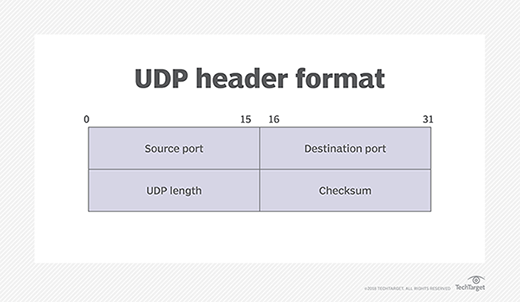
\includegraphics[width=\textwidth]{Images/networking-udp_mobile.png} 
\vspace{-0.3cm} 
\caption{Format eines UDP-Datagramm Headers.}
\label{fig-elise} 
\end{figure}
Hierbei gibt Sourceport die Port-Nummer des sendenden Prozesses an, dies wird benötigt, falls der Empfänger auf das Paket antworten soll. Ist dies nicht der Fall kann dieser Wert aber auch Problemlos auf 0 gesetzt werden. Der Destination port gibt den Prozess an, der das Paket empfangen soll. UDP lenght gibt die Länge des jeweiligen Datagramms, also die Länge von Header + Daten, an. Checksum ist die (optionale) Prüfsumme, dieser Wert wird wenn nicht verwendet auf 0 gesetzt. Gefolgt wird der Header dann von den eigentlichen Nutzdaten (in engl. auch als Payload bezeichnet). Für die eigentliche Übertragung des UDP-Pakets ist das Internet Protokoll(IP) vorgesehen, wodurch dem Paket noch ein weiter Header vorgesetzt wird,  in welchen sich die von dem Internet Protokoll benötigten Daten befinden [Abbildung 2.4.2]

\begin{figure}[H] \centering
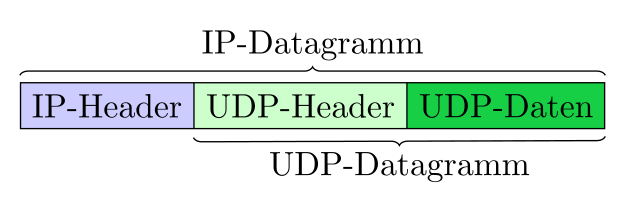
\includegraphics[width=\textwidth]{Images/Udp-package-scheme.png} 
\vspace{-0.3cm} 
\caption{Vollständiges zu übertragendes Paket.}
\label{fig-elise} 
\end{figure}